\documentclass[12pt,hyperref]{labbook}
\usepackage[utf8]{inputenc}
\usepackage{graphicx}
\usepackage[margin=1.0in]{geometry}
\usepackage{setspace}
\usepackage{listings}
\usepackage{color}
\usepackage{array}
\usepackage{hyperref}
\usepackage[]{algorithm}
\usepackage[noend]{algpseudocode}
\usepackage{csquotes}

\newcolumntype{P}[1]{>{\centering\arraybackslash}p{#1}}

\definecolor{dkgreen}{rgb}{0,0.6,0}
\definecolor{gray}{rgb}{0.5,0.5,0.5}
\definecolor{mauve}{rgb}{0.58,0,0.82}

\textwidth=16.5cm

\lstset{frame=tb,
  language=C++,
  aboveskip=3mm,
  belowskip=3mm,
  showstringspaces=false,
  columns=flexible,
  basicstyle={\small\ttfamily},
  numbers=none,
  numberstyle=\tiny\color{gray},
  keywordstyle=\color{blue},
  commentstyle=\color{dkgreen},
  stringstyle=\color{mauve},
  breaklines=true,
  breakatwhitespace=true,
  tabsize=3
}

\title{Notes for Undergraduate Research Work}
\author{Hollis Bui}

\begin{document}

\maketitle
\newpage
\tableofcontents
\newpage

\labday{General}

\experiment{R Notes}

Remember: R is 1-indexed.

Format of If/Else:

\noindent\begin{minipage}{\linewidth}
\begin{lstlisting}
if {

}else{

}
\end{lstlisting}
\end{minipage}

In R-Studio, you can multiline comment (and uncomment) by pressing
CTR + SHIFT + C

To check current directory in R, type in and execute \enquote{getwd()}.

\experiment{TODOs}

\begin{enumerate}
    \item PANSE model implentation:
    \begin{enumerate}
        \item PANSEParameter.cpp
        \item PANSEModel.cpp
        \item PANSEParameter.h
        \item PANSEModel.h
        \item Ask about sigma term -- Done
        \item Ask about lambda prime term (is it lambda prime?) — check RFP section for how to actually calculate — DONE
    \end{enumerate}
    \item Expand Unit Testing:
    \begin{enumerate}
        \item Test Cov Matrixes — STALLED: Still need final two
        \item Test MCMC - STALLED: Need run, varyInitialConditions, calculateGewekeScore, getLogLikelihoodPosteriorMean, and setRestartFileSettings as well as two test that only functions.
        \begin{itemize}
            \item Implement other unit testing first
        \end{itemize}
        \item Parameter -- In progress
        \item Test RFP Parameter
        \item Test Trace
        \item ...Per class basis
        \item Eventually, some R scripts to do a short run for each model: Talk to Cedric
    \end{enumerate}
    \item r
    \item When working with gene-specific parameters, the openmp statements aren’t working (memory is such a mess in the area) — break down parallelization, try to find where the issue is. Perhaps start with dynamic arrays, change to vectors. Gabriel thinks the slowdown from vectors in general is made up by better parallelization in avoiding dynamic arrays.
    \begin{itemize}
        \item —STALLED. Literally can’t test speeds of various optimizations and cores right now.
    \end{itemize}
    \item Documentation
\end{enumerate}

\labday{May 13, 2016 Notes}

\experiment{PANSE Concepts}

\begin{figure}[h!]
    \center
    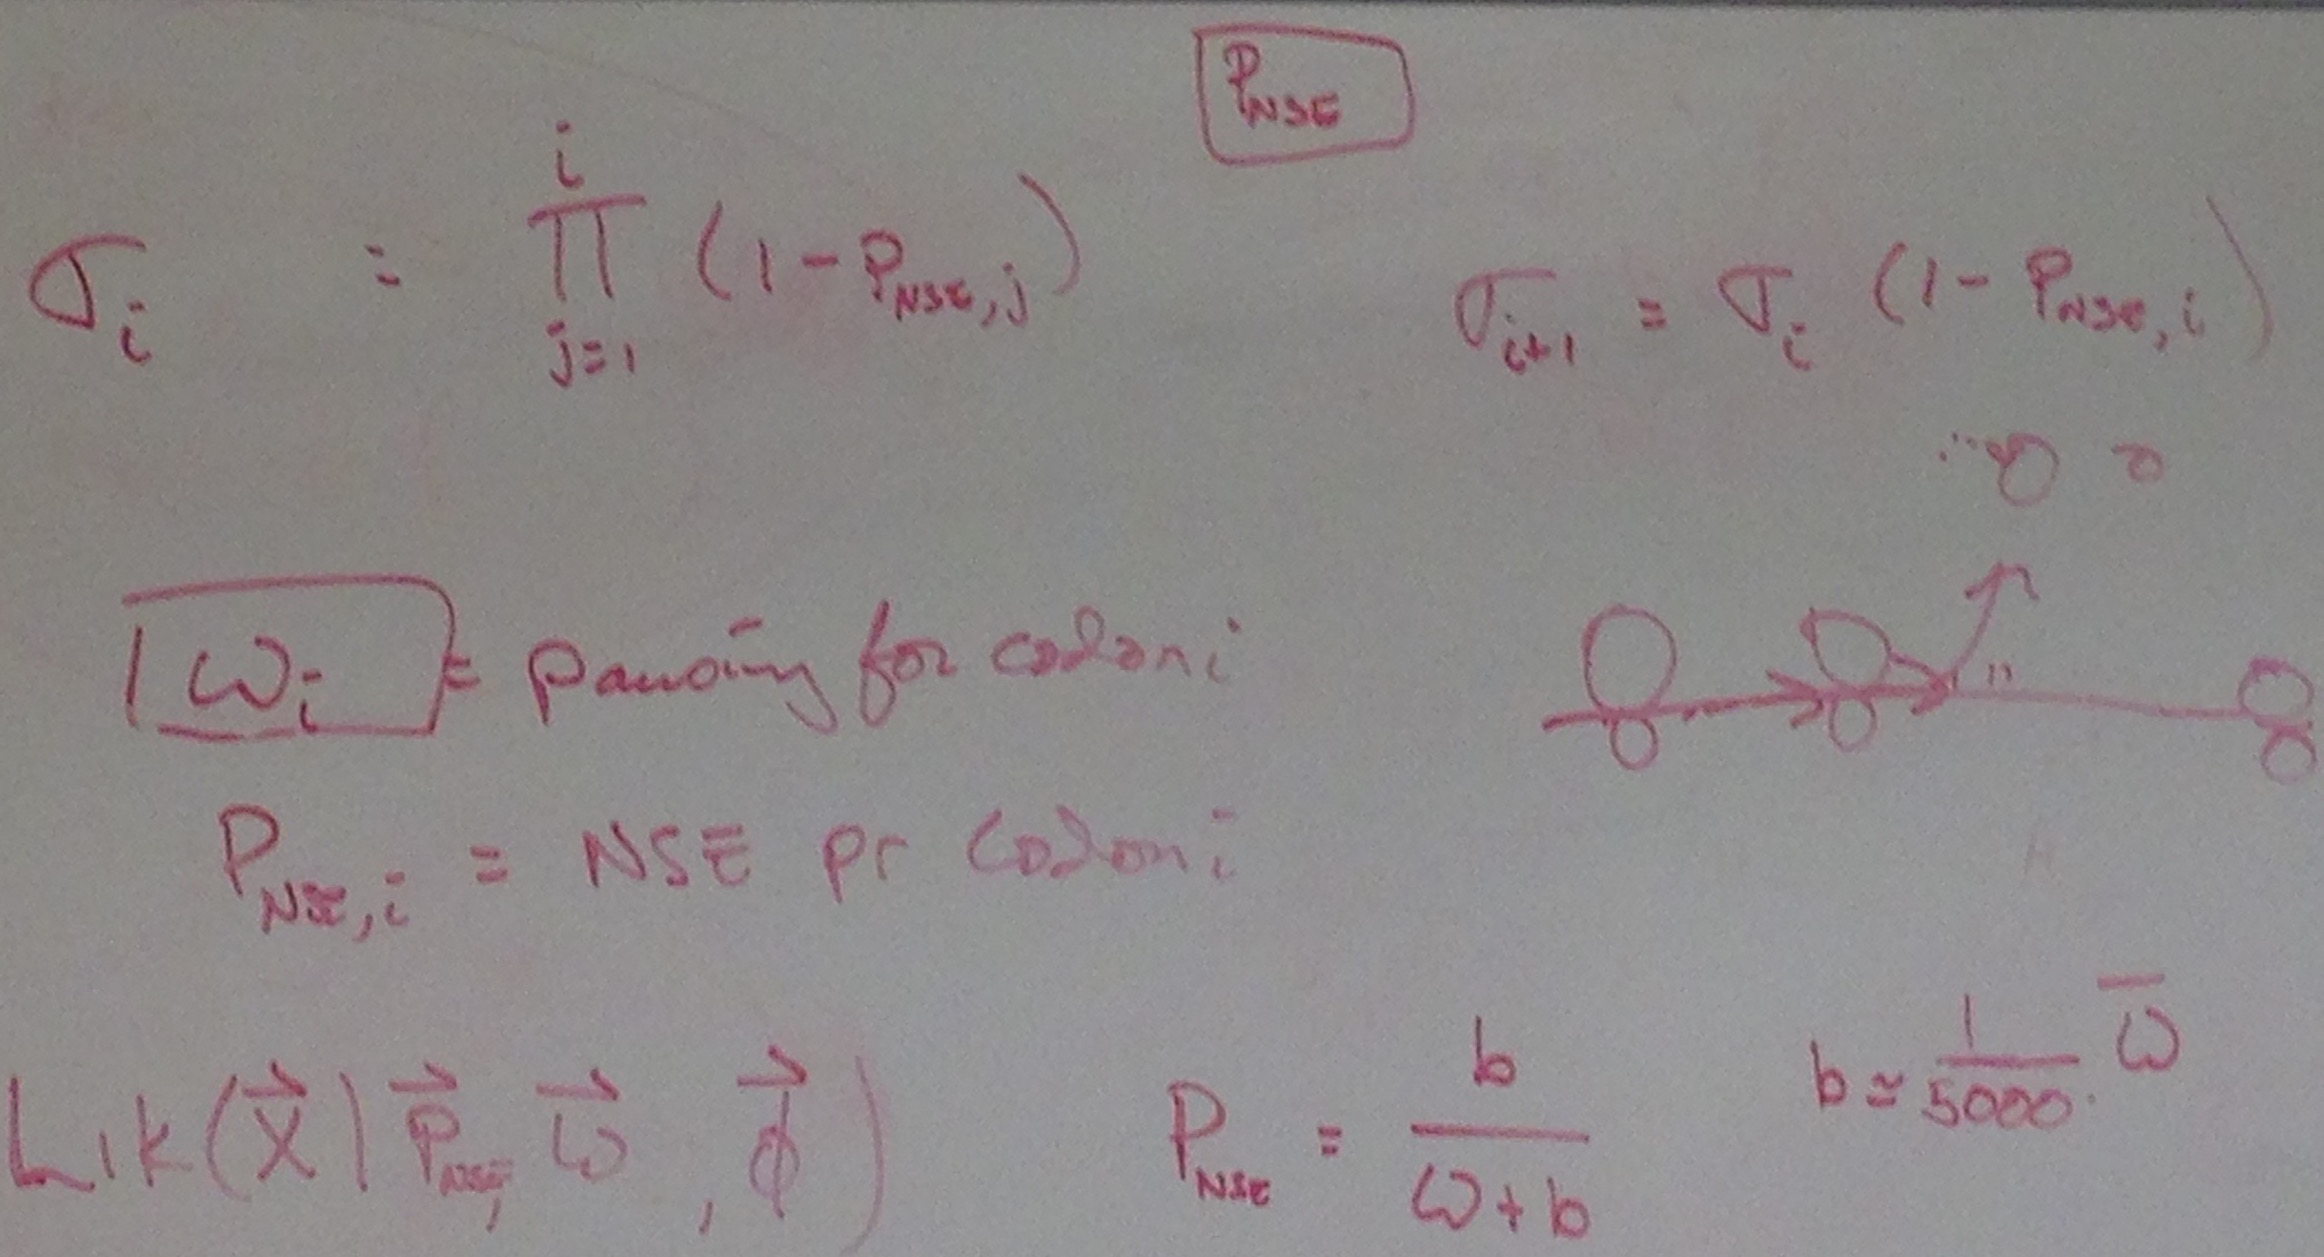
\includegraphics[width=\textwidth,keepaspectratio]{5-13-16img.jpg}
    \label{figure}
\end{figure}

\begin{equation}
    \sigma_{i} = \prod_{j=1}^{i} (1 - P_{NSE,j})
\end{equation}

$\omega_i$ = pausing for codon i

$p_nse, i$  = NSE $\Pr$ (probability) for codon i

This is codon-based.

Likelihood of the data given the parameters: 
$\mathcal{L}(\vec{x}|\vec{P_{NSE}},\vec{\omega}, \vec{\phi})$

Will be a much smaller data set, and with hundreds of calculations rather than thousands.

Randomly select $\sim$600 genes instead of 5400

Sigma vector of: $\sigma_{i + 1} = \sigma_i (1 - P_{NSE, i})$

Function is of probability of getting there vs waiting time once there

\experiment{TODOs}

\begin{itemize}
    \item Getting pausing values with simpler models (ROC)
    \item First analysis could be just estimating these terms
    \item This would mean creating a simulated data set.
    \item For simulation: $P_{NSE} = \frac{b}{\omega + b}$, where b is on the order of 1/5000 times average omega. ($b \simeq \frac{1}{5000}\overline{\omega}$) Talk to Jeremy about this, he may have finished this by now.
\end{itemize}

See the 2015 paper, 2011 paper with primal

\labday{May 19, 2016 Notes}

\experiment{PANSE Concepts}

rfp.model.pdf:
Reasoning [for lambda] is that for the sampling the Boltsman coefficient. See the explanation around equation (4) and the Z’s and Y’s.

Lambda Prime = Lambda.c * Z / Y, or call it K.

$\lambda^{\prime} = \lambda_c * \frac{Z}{Y}$

Z is the overall state space

Y is what is sampled

$\lambda_c = \lambda^{\prime} * \frac{C}{K}$. Let K be a new independent parameter, and keep track of Lambda Prime.

\labday{May 25, 2016 Notes}

\experiment{PANSE Concepts}

Codon-Specific Elongation Rate:
$P_{NSE} = \frac{b}{b + c}$ where b is where it flies off and c is where it continues.

Omega is the odds ratio of $\frac{P_{NSE}}{1 - P_{NSE}}$. Therefore $\omega = \frac{b}{c}$

Look at 2006, 2007 papers.

LOOK AT UPDATED PDF: IT’S IN FRAMEWORK

Psi (the symbol which I *thought* was Omega)
is the ribosome initiation rate: Rate at which ribosomes are jumping onto the mRA. Phi is the rate that they are jumping off at the very end.

If you have 50\% chance to get to the end, then Psi is twice as long as Phi

Phi = Psi * Sigma.

Don’t redo calculations from scratch, but rather in series.

\experiment{Parallelization}

\begin{itemize}
    \item Only 20 AA’s — Only 20 cores to spread load unto
    \item AA’s with 6 codons of course take more time than those with 2
\end{itemize}

Gilchrist thinks what is meant by Gene-Specific Parameters is to parallelize at the highest level, 
i.e. at the gene or amino acid level.

I should check the code; find where the OpenMP statements are etc

Mostly something to ask other people about if I want to tackle the problem.

\labday{May 26, 2016 Notes}

\experiment{Parallelization}

Cedric's input:
\begin{itemize}
    \item phi calculation, with mcmc accept/reject
    \item dynamic arrays
    \item big loop around everything
    \item code doesn’t work
    \item couldn’t figure out why
    \item didn’t spend that much time
\end{itemize}

we ended up parallelizing in the model class:

calculateLogLikelihoodRatioPerGene, apparently doesn’t do much.
Perhaps better to parallelize outside, with the big loop

Run a ROC model, then RFP

I’m running a fasta file that is simulated, so I know that it is true

I kinda need the R side

Get to the point where we suspect memory is the problem

Dynamic Arrays -\textgreater Vectors

\labday{May 31, 2016 Notes}

\begin{itemize}
    \item Start 1:21
    \item break 3:19
    \item back 3:24
    \item break 4:55
    \item return 5:02
    \item end 7:02
\end{itemize}

2 + 1.5 + 2

\experiment{Parallelization}

Go ahead and replace dynamic arrays with vectors, first

And then do this barebones calculation of runs to see if it makes it faster,
without regards to parallelization.

\labday{June 1, 2016 Notes}

\begin{itemize}
    \item Start 1:30
    \item Break 3:30
    \item Return 3:35
    \item End 7:00
\end{itemize}

2 + 3.5

\experiment{Parallelization}

From yesterday:

\noindent\begin{minipage}{\linewidth}
\begin{lstlisting}
0.00621732 - 10
0.00687881 - 100
0.00947537 - 1000
0.00713974 - 10000
0.00785908 - 10000
0.00750889 - 10
\end{lstlisting}
\end{minipage}

For today:

\noindent\begin{minipage}{\linewidth}
\begin{lstlisting}
0.0572747 - 10
0.0698414 - 100
\end{lstlisting}
\end{minipage}

…Odd, 10x as long on average

The above was in DEBUG mode. Release mode redos:

\begin{table}[H]
    \centering
    \begin{tabular}{|c|c|c|c|}
        \hline
        \textbf{A or V} & \textbf{Runs} & \textbf{Modifiers} & \textbf{Avg Time} \\
        \hline
        V & 100 & & 0.0141421 \\
        A & 100 & & 0.0047742 \\
        V & 10000 & & 0.00850093 \\
        A & 10000 & & 0.00479609 \\
        V & 10000 & No Deletion & 0.00871843 \\
        A & 10000 & No Deletion & 0.00491614 \\
        V & 10000 & std::sort & 0.00841396 \\
        \hline
        A & 10000 & & 0.00598796 \\
        A & 10000 & & 0.00520682 \\
        A & 100000 & & 0.00455916 \\
        A & 100000 & std::sort & 0.00776886 \\
        V & 100000 & & 0.00795495 \\
        V & 100000 & std::sort & 0.00785736 \\
        \hline
        A & 100000 & std::sort & 0.00383634 \\
        A & 100000 & & 0.00385638 \\
        A & 100000 & std::sort & 0.00392021 \\
        \hline
    \end{tabular}
\end{table}

Note: Vectors are ~2x as long on average now

\experiment{PANSE Implementation}

Next step: Make a list of everything PANSE touches and unit test these things (first and foremost before actually writing PANSE)

ALSO: Estimate and track how long, in reality, it takes to do each unit testing

PARFP, PTRFP? Just calling it RFP might be misleading.

\labday{June 2, 2016 Notes}

\begin{itemize}
    \item Start 1:01
    \item Break 3:35
    \item Return 3:50
    \item End 6:58
\end{itemize}

Spent till 4 (3 hours) compiling notes and creating a git directory.

\experiment{PANSE Implementation}

Expecting to spend ~1 hour deciding on what PANSE will need (or, rather, what RFP will need).

Talk with Gilchrist:

So data position feeds into:
\begin{itemize}
    \item a) data on gene 
    \begin{itemize}
        \item ab) to feed into ROC-RFP
    \end{itemize}
    \item or b) PANSE-RFP
\end{itemize}

\experiment{Lareau Data}
Which file type should I be reading in? RFP or Fasta?

For sample data for PANSE:

Lareau Paper -\textgreater GSE -\textgreater The untreated replicates 1,2,3. Take one, and even then only a subset of 
one of them as sample data.

The Lareau material may have undergone more processing that the new Weinberg GSE published Feb 10 2016. 

\enquote{Start with Lareau paper data} -- Gilchrist, 5:33

\labday{June 3, 2016 Notes}

\begin{itemize}
    \item Start 1:35
    \item Break 4:09
    \item Return 4:14 
\end{itemize}

\experiment{Lareau Data}

Decided to start reading the Lareau material. Began by looking directly at definition of data set
(I chose untreated replicate 1) and then parse the data to get a smaller subset (file size otherwise
is too large at 35MB)

Took longer than expected... When files finally parsed, 5:45.

Now have a data set of size 400 KB: those genes with 11 to 100 (inclusive) codons. 

\labday{June 6, 2016 Notes}

\experiment{TODOs}

Immediate future goals:
\begin{enumerate}
    \item Generate new Lareau material following specifications of Gilchrist talk, below.
    \item Just work, from now on, with the labbook class. Don't have to reformat old content.
    \item Formally write up a list of things TODO with Unit Testing for Parameter
    \item Unit Test up-to-date with Parameter
    \item Write up pseudo-code with PANSE itself to prepare for it
    \item Create and test a function for reading in Lareau material (low priority)
    \item Parallelization is after the initial PANSE stuff is implemented, very low priority
\end{enumerate}

\experiment{Lareau Data}

Talk with Gilchrist:

Let's get a randomly distributed set of data rather straight up isolation.

See below for how to randomly distribute; want only 100 genes.

61 Parameters Pausing Time

Lots of gene-specific parameters that scale with each gene.

Let's say average of each gene is ~300 AAs.

So ~7 observations per gene.

Try to get 2 parameters for a fair amount of information. Calculating at sigma is going increase at
gene length.

And of course longer gene sequences take longer to parse.

So probably want a data base for playing around with of 100 genes, between 200 and 400 AAs long

Do we need to test with all 61 parameters?
2-codon AA's are the quickest thing to work with. 

So may want to start with 100 genes of 200-400 AAs
Estimate these parameters with a small subset of the codons, starting with the 2-codon ones.
If they are behaving properly, scale up to 3/4/etc.

\noindent\makebox[\linewidth]{\rule{\paperwidth}{0.4pt}}

Long is de-facto standard
Lareau argues that Short is also relevant despite usually being thrown out

Long and short: tell how elongation is at each position.
Our model is based on pausing. 

So how do long and short factor in? Well, we don't know yet.

We could base it on just one or the other or combine the two.

For now let's just base it on Long.

\noindent\makebox[\linewidth]{\rule{\paperwidth}{0.4pt}}

After about thirty minutes following the talk with Gilchrist -- new 
subset of data produced via modifying old Perl scripts. Now have the specified data set
in the final \enquote{finalData.txt} -- 516 KB.

Interestingly small size -- seems like old data set had that many genes of smaller AA length.

\noindent\makebox[\linewidth]{\rule{\paperwidth}{0.4pt}}

Spent an hour afterward reading over labbook documentation and reformatting notes where needed.

\labday{June 7, 2016 Notes}
In the course of running an RFP Model, the following functions are called (and have yet to be
unit tested).

\experiment{TODOs}

\begin{itemize}
    \item initParameterSet (actually already done... mostly) -- general parameter
    \begin{itemize}
        \item test std\_csp changes -- Done
        \item test numAcceptForCodonSpecificParameters changes -- Done
        \item Possibly setNumMutationSelectionValues -- Ignore for now
        \item Possibly initCategoryDefinitions --Ignore for now
        \item For the two above -- Find how to check delM and delEta of category (a vector of Mixture Definitions) -- Done
        \item Check many final changes at the end of this function -- Three remaining
    \end{itemize}
    \item initRFPParameterSet -- RFP exclusive
    \item getSelectionCategory -- general parameter -- Done
    \item InitializeSynthesisRate -- general parameter
    \begin{itemize}
        \item calculateSCUO
        \item quickSortPair
        \item quickSort
        \item Parameter::randLogNorm
    \end{itemize}
    \item setParameter -- RFP model exclusive
    \item mcmc.run -- MCMC function on RFP(TODO later?)
\end{itemize}

\experiment{Unit Testing}

Going to take it one step at a time, finish up initParameterSet testing...

Finished most of initParameterSet completely. Need to ask Cedric about a duplicate function before
finishing the final two functions.

May need to write a function to unit test with the categories variable itself, but
all that happens otherwise is it pushes unto the vector of vector of vectors.

Encountering a strange printing bug right before the end. While if statement works correctly,
the final confirmation of initParameterSet isn't being printed.

Example output:

\noindent\begin{minipage}{\linewidth}
\begin{lstlisting}
Parameter getMixtureAssignment --- Pass
Parameter setMixtureAssignment --- Pass
Parameter getMutationSelectionState --- Pass
Parameter getNumParam --- Pass
Parameter getNumMixtureElements --- Pass
Parameter getStdDevSynthesisRate --- Pass
Parameter setStdDevSynthesisRate --- Pass
Parameter getCurrentStdDevSynthesisRateProposalWidth --- Pass
Parameter getNumAcceptForStdDevSynthesisRate --- Pass
Parameter getStdCspForIndex --- Pass
Parameter getNumAcceptForCspForIndex --- Pass
Parameter getNumMutationCategories --- Pass
Parameter getNumSelectionCategories --- Pass
Parameter getMutationCategory --- Pass
Parameter getSelectionCategory --- Pass
Parameter getMixtureElementsOfMutationCategory --- Pass
Parameter getMixtureElementsOfSelectionCategory --- Pass
Parameter getCategoryProbability --- Pass
Parameter setCategoryProbability --- Pass
Parameter getSynthesisRate --- Pass
Parameter setSynthesisRate --- Pass
Parameter getSynthesisRateProposalWidth --- Pass
0
Parameter initParameterSet --- Pass

Process finished with exit code 0
\end{lstlisting}
\end{minipage}

vs

\noindent\begin{minipage}{\linewidth}
\begin{lstlisting}
Parameter getMixtureAssignment --- Pass
Parameter setMixtureAssignment --- Pass
Parameter getMutationSelectionState --- Pass
Parameter getNumParam --- Pass
Parameter getNumMixtureElements --- Pass
Parameter getStdDevSynthesisRate --- Pass
Parameter setStdDevSynthesisRate --- Pass
Parameter getCurrentStdDevSynthesisRateProposalWidth --- Pass
Parameter getNumAcceptForStdDevSynthesisRate --- Pass
Parameter getStdCspForIndex --- Pass
Parameter getNumAcceptForCspForIndex --- Pass
Parameter getNumMutationCategories --- Pass
Parameter getNumSelectionCategories --- Pass
Parameter getMutationCategory --- Pass
Parameter getSelectionCategory --- Pass
Parameter getMixtureElementsOfMutationCategory --- Pass
Parameter getMixtureElementsOfSelectionCategory --- Pass
Parameter getCategoryProbability --- Pass
Parameter setCategoryProbability --- Pass
Parameter getSynthesisRate --- Pass
Parameter setSynthesisRate --- Pass
Parameter getSynthesisRateProposalWidth --- Pass


Process finished with exit code 0
\end{lstlisting}
\end{minipage}

\labday{June 8, 2016 Notes}

\experiment{Unit Testing}

Started by writing and testing a function for numAcceptForSynthesisRate.

Printing this statement seems to have fixed the odd print bug mentioned yesterday.

After doing that, I decided to write up on the documentation of Unit Testing I have done so far.

Asked Cedric about getSelectionCategory and getSynthesisRateCategory (paraphrased):

\begin{displayquote}
It's related to how we may have delta and Phi values...

We are trying to find out how efficient your codons have to be to reach a production rate
assuming cost is constant.

Cost = Benefit * production rate (Phi)

Switching to a different selection environment:
Different cost, different benefit, and therefore different Phi.

If you have 2 selection categories, you have to have two synthesis categories. 
They are the same even if we don't know them, but it saves renaming it to something more general.
\end{displayquote}

Finally finished initParameterSet besides checking categories matrix itself (minor, to do later).

Continued TODO:

\experiment{TODOs}

\begin{itemize}
    \item initRFPParameterSet -- RFP exclusive
    \item InitializeSynthesisRate -- general parameter
    \begin{itemize}
        \item calculateSCUO
        \item quickSortPair
        \item quickSort
        \item Parameter::randLogNorm
    \end{itemize}
    \item setParameter -- RFP model exclusive
    \item mcmc.run -- MCMC function on RFP(TODO later?)
\end{itemize}

Next goals: Do the internal functions for InitializeSynthesisRate related to quickSort.

Finish up InitializeSynthesisRate.

\labday {June 9, 2016 Notes}

Began by checking github; fixed semicolon error and confirmed package worked correctly.

\experiment{TODOs}

To truly finish testing InitializeSynthesisRate, we would need:

\begin{itemize}
    \item calculateSCUO
    \item Parameter::randLogNorm
    \item quickSortPair
    \begin{itemize}
        \item pivotPair
        \begin{itemize}
            \item swap (doubles)
        \end{itemize}
    \end{itemize}
    \item quickSort
    \begin{itemize}
        \item pivot
        \begin{itemize}
            \item swap (ints)
        \end{itemize}
    \end{itemize}
\end{itemize}

Ask Cedric if it'd be a good idea to just use std::sort instead of quickSort.

The quick sort algorithms are very math-intensive, so Unit Testing them may be lower priority.

For now, I am switching to unit testing RFP-exclusive functions.

\begin{itemize}
    \item initRFPParameterSet (in RFPParameter.cpp)
    \begin{itemize}
        \item check currentCodonSpecificParameter
        \item check proposedCodonSpecificParameter
        \item check lambdaValues (optional -- currently unused variable)
        \item check numParam -- Done
        \item check bias\_csp -- always set to 0, can ignore for now
        \item check std\_csp -- Done
        \item check groupList -- Done
    \end{itemize}
    \item setParameter (in RFPModel.cpp) -- may be untestable, ignore for now
\end{itemize}

In the course of working on checking RFPParameter, wrote up Unit Testing for all
Group List functions in Parameter.cpp

May need a wrapper function for currentCodonSpecificParameter and proposedCodonSpecificParameter
extraction. Talk to Cedric.

Refocusing overall goals:
\begin{enumerate}
    \item Unit Test up-to-date with Parameter
    \begin{itemize}
        \item{initRFPParameterSet}
        \begin{itemize}
            \item check currentCodonSpecificParameter -- stalled, ask Cedric
            \item check proposedCodonSpecificParameter -- stalled, ask Cedric
        \end{itemize}
        \item{InitializeSynthesisRate}
        \begin{itemize}
            \item calculateSCUO
            \item Parameter::randLogNorm
            \item quickSortPair
            \begin{itemize}
                \item pivotPair
                \begin{itemize}
                    \item swap (doubles)
                \end{itemize}
            \end{itemize}
            \item quickSort
            \begin{itemize}
                \item pivot
                \begin{itemize}
                    \item swap (ints)
                \end{itemize}
            \end{itemize}
        \end{itemize}
        \item mcmc::run -- MCMC function on RFP
    \end{itemize}
    \item Write up pseudo-code with PANSE itself to prepare for it
    \item Create and test a function for reading in Lareau material (low priority)
    \item Parallelization is after the initial PANSE stuff is implemented, very low priority
\end{enumerate}

TODO tomorrow:

Ask about current/proposed CSP Parameter, quicksort vs std::sort, and how (if) to unit test
the more computation-intensive functions.

Finally replace cout statements in my own section of main.

Begin testing with MCMC run while waiting for others to arrive.

\labday {June 10, 2016 Notes}

There exists a heirarchy of functions to test before finally testing mcmc.run. Test the
subitems first: (NOTE: Testing with RFPModel)
\begin{itemize}
    \item mcmc::run
    \begin{itemize}
        \item mcmc::varyInitialConditions
        \begin{itemize}
            \item model::proposeCodonSpecificParameter -- wrapper to RFPparameter
            \item model::proposeHyperParameters -- parameter::proposeStdDevSynthesisRate
            \item model::proposeSynthesisRateValues -- wrapper to parameter
            \item model::getGroupListSize -- wrapper to parameter (done?)
            \item model::getGrouping -- wrapper to parameter (done?)
            \item model::updateCodonSpecificParameter -- wrapper to RFPparameter
            \item model::updateAllHyperParameter -- just calls updateStdDevSynthesisRate -- Ask
            \begin{itemize}
                \item updateStdDevSynthesisRate -- wrapper to parameter
            \end{itemize}
            \item model::getNumSynthesisRateCategories -- wrapper to parameter (done?)
            \item model::getSynthesisRateCategory -- wrapper to parameter (done?)
            \item model::getSynthesisRate -- wrapper to parameter (done?)
            \item model::getMixtureAssignment -- wrapper to parameter (done?)
            \item model::getStdDevSynthesisRate -- wrapper to parameter (done?)
            \item parameter::densityLogNorm
            \item paramter::randExp
            \item model::updateSynthesisRate -- wrapper to parameter
            \item model::updateGibbsSampledHyperParameters -- does not do anything
        \end{itemize}
        \item model::setNumPhiGroupings -- wrapper to parameter::setNumObservedPhiSets (done?)
        \item model::initTraces -- wrapper to RFPparameter initAllTraces
        \item model::updateTracesWithInitialValues
        \begin{itemize}
            \item parameter::updateSynthesisRateTrace
            \item parameter::updateMixtureAssignmentTrace
            \item RFPparameter::updateCodonSpecificParameterTrace
        \end{itemize}
        \item model::setLastInteration -- wrapper to parameter (done?)
        \item model::writeRestartFile -- wrapper to RFPparameter writeEntireRestartFile
        \item model::printHyperParameters -- uneeded to test, just prints
        \item model::getNumMixtureElements -- wrapper to parameter (done?)
        \item mcmc::acceptRejectCodonSpecificParameter
        \begin{itemize}
            \item model::calculateLogLikelihoodRatioPerGroupingPerCategory
            \item model::updateCodonSpecificParameterTrace
        \end{itemize}
        \item model::adaptCodonSpecificParameterProposalWidth -- wrapper to RFPparameter
        \item mcmc::acceptRejectHyperParameter
        \begin{itemize}
            \item model::calculateLogLikelihodRatioForHyperParameters
            \item model::updateHyperParameter -- parameter::updateStdDevSynthesisRate
            \item model::updateHyperParameterTraces
        \end{itemize}
        \item model::adaptHyperParameterProposalWidths -- calls adaptStdDevSynthesisProposalWidth,
        a wrapper to parameter. Uses traces.
        \item mcmc::acceptRejectSynthesisRateLevelForAllGenes
        \begin{itemize}
            \item model::getMixtureElementsOfSelectionCategory -- wraps parameter (done?)
            \item model::calculateLogLikelihoodRatioPerGene
            \item model::getCategoryProbability -- wrapper to parameter (done?)
            \item parameter::randMultinom
            \item model::setMixtureAssignment -- wrapper to parameter (done?)
            \item model::updateSynthesisRateTrace
            \item model::updateMixtureAssignmentTrace
            \item model::calculateAllPriors -- currently does nothing
            \item parameter::randDirichlet
            \item model::setCategoryProbability -- wrapper to parameter (done?)
            \item model::updateMixtureProbabilitiesTrace
        \end{itemize}
        \item model::adaptSynthesisRateProposalWidth -- wrapper to parameter
        \item mcmc::calculateGewekeScore
    \end{itemize}
\end{itemize}

TODO:

Ask about why it is that Hyper Parameters == StdDevSynthesisRate, always

Don't know if we need to test wrapper functions i.e. those in Model that simply perform
a function in its associated Parameter object.

Ask about why dynamic arrays were in code in the first place, i.e. in randMultinom.

New modified list stripping out some things that are more-or-less done
(Or those that depend on unimplemented functions or those with random variables):
\begin{itemize}
    \item mcmc::run
    \begin{itemize}
        \item mcmc::varyInitialConditions
        \item model::initTraces -- wrapper to RFPparameter initAllTraces
        \item model::updateTracesWithInitialValues
        \begin{itemize}
            \item parameter::updateMixtureAssignmentTrace
            \item RFPparameter::updateCodonSpecificParameterTrace
        \end{itemize}
        \item model::writeRestartFile -- wrapper to RFPparameter writeEntireRestartFile
        \begin{itemize}
            \item parameter::writeBasicRestartFile
            \item writeRFPRestartFile
        \end{itemize}
        \item mcmc::acceptRejectCodonSpecificParameter
        \begin{itemize}
            \item model::calculateLogLikelihoodRatioPerGroupingPerCategory
            \item model::updateCodonSpecificParameterTrace
        \end{itemize}
        \item model::adaptCodonSpecificParameterProposalWidth --
        wrapper to RFPparameter. Uses traces.
        \item mcmc::acceptRejectHyperParameter
        \begin{itemize}
            \item model::calculateLogLikelihodRatioForHyperParameters
            \item model::updateHyperParameter -- parameter::updateStdDevSynthesisRate
            \item model::updateHyperParameterTraces
        \end{itemize}
        \item model::adaptHyperParameterProposalWidths -- calls adaptStdDevSynthesisProposalWidth,
        a wrapper to parameter. Uses traces.
        \item mcmc::acceptRejectSynthesisRateLevelForAllGenes
        \begin{itemize}
            \item model::calculateLogLikelihoodRatioPerGene
            \item model::updateSynthesisRateTrace
            \item model::updateMixtureAssignmentTrace
            \item model::updateMixtureProbabilitiesTrace
        \end{itemize}
        \item model::adaptSynthesisRateProposalWidth -- wrapper to parameter. Uses traces.
        \item mcmc::calculateGewekeScore
    \end{itemize}
\end{itemize}

After writing the setNumObservedPhiGroupings and lastIteration unit testing functions and
updating these notes, worked on restart file writing.

TODO: Discuss with Cedric how to proceed to unit testing with restart files
in the future, i.e. keep in same function or separate.

Next step:

Probably work with traces. Not sure how to proceed with unit testing
the most complicated functions re: computation, nor with reading/writing files yet.

\labday {June 11, 2016 Notes}
Mostly read documentation. Worked from home, so no benefit of discussing implementation topics.
Worked less than planned.

\labday {June 13, 2016 Notes}
Discussing Unit Testing with Cedric:

OK'd changing quicksort (simple implementation) to std::sort.

Instead of running the higher-level functions that are directly used, 
probably better to stick to the simple functions and then test mcmc algorithm runs with
100 samples; compare the likelihoods of each model, which should be similar, to detect errors.

For the intense calculations, for now ignore. The calculation unit tests will be summed up (in a
general sense) by just doing mcmc algorithm runs.

First, going to change std::sort.

After that was done, decided to clean up some R-side unit testing in preparation of testing
mcmc algorithm runs -- since in R you can set seed for entire C-side implementation.

\experiment{TODOs}
\begin{itemize}
    \item Fix the TODO note in Parameter.cpp under initParameterSet
    \item Ask Cedric about:
    \begin{itemize}
        \item Testing restart files: keep in same function or separate unit tests.
        \item May need a wrapper function for currentCodonSpecificParameter and proposedCodonSpecificParameter extraction. 
        \item How to actually run R-side scripts; weird error messages.
        \item What is the inst folder? Can we remove it, since it seems to be old Unit Testing Data stuff?
    \end{itemize}
\end{itemize}

Still need to look at Trace stuff as next major step without help from Cedric.

Spend at most two more days on Unit Testing at this rate; after, will start thinking solely
on PANSE.

\labday {June 14, 2016 Notes}

Yesterday ended by running memory leak checks in the background on a whim due to debugging
some new calls without associated delete calls.

Found a confirmed memory leak with my\_print. Started today by flushing output on
both C and R side of code, as well as expanding unit testing for Utility.h.

Spent an hour and a half on this.

Came in late, could not ask Cedric questions.

\experiment{Traces}
Order of Trace functions to examine in a typical model run (via MCMC::run):
\begin{itemize}
    \item model::initTraces(samples + 1, genome.getGenomeSize());
    \begin{itemize}
        \item RFPparameter->initAllTraces
        \begin{itemize}
            \item traces.initializeRFPTrace (RFP-only)
            \begin{itemize}
                \item initializeSharedTraces
                \item initCodonSpecificParameterTrace (for both alp and lmPri)
            \end{itemize}
        \end{itemize}
    \end{itemize}
    \item model::updateTracesWithInitialValues(genome) -- TO BE EXAMINED
    \begin{itemize}
        \item parameter::updateSynthesisRateTrace
        \begin{itemize}
            \item traces.updateSynthesisRateTrace
        \end{itemize}
        \item parameter::updateMixtureAssignmentTrace
        \begin{itemize}
            \item traces.updateMixtureAssignmentTrace
        \end{itemize}
        \item RFPparameter::updateCodonSpecificParameterTrace
        \begin{itemize}
            \item traces.updateCodonSpecificParameterTraceForCodon (for alp and lmPri)
        \end{itemize}
    \end{itemize}
    \item mcmc::acceptRejectCodonSpecificParameter
    \begin{itemize}
        \item model::calculateLogLikelihoodRatioPerGroupingPerCategory
        \item model::updateCodonSpecificParameter(grouping)
        \item model::updateCodonSpecificParameterTrace
    \end{itemize}
    \item model::adaptCodonSpecificProposalWidth -- wrapper to RFPparameter. Uses traces
    \item mcmc::acceptRejectHyperParameter
    \begin{itemize}
        \item model::calculateLoglIkelihoodRatioForHyperParameters
        \item model::updateHyperParameter - parameter::updateStdDevSynthesisRate
        \item model::updateHyperParameterTraces
    \end{itemize}
    \item model::adaptHyperParameterProposalWidths - calls adaptStdDevSynthesisProposalWidth,
    a wrapper to parameter. Uses traces.
    \item mcmc:acceptRejectSynthesisRateLevelForAllGenes
    \begin{itemize}
        \item model::calculateLogLikelihoodRatioPerGene
        \item model::updateSynthesisRateTrace
        \item model::updateMixtureAssignmentTrace
        \item model::updateMixtureProbabilitiesTrace
    \end{itemize}
    \item model::adaptSynthesisRateProposalWidth -- wrapper to parameter. Uses traces.
\end{itemize}

This list is still incomplete, but we shall start implementing now for convenience.

Need to keep examining functions... Ended before checking model::updateTracesWithInitialValues

\labday {June 15, 2016 Notes}

Answers to Cedric questions:
\begin{itemize}
    \item In general, design of code is up to me. Seems good with whatever.
    \item DevRScripts are super out-dated. Be careful of what to use, i.e. a lot of functions
    are using old definitions and need additional arguments.
    \item Again, for overall unit testing:
    \begin{itemize}
        \item Do a run, know what the output is.
        \item 
        Then repeat that run in the testThat function, compare the two runs. As long as outputs are the same, everything is fine.
    \end{itemize}
    \item Good scripts to base code off of: allUnique scripts.
    Specifically allUnique\_kl\_reduced.R, allUnique\_simMod.R
    \item Bad script: runROCModelFromGoodValues.R
\end{itemize}

Cedric commented that there was a lot of old and outdated files, so I spent some time
trying to clean up the more obvious files.

\begin{itemize}
    \item Removed inst folder from RibModelFramework.
    \item Removed cleanSeq() finally
    \item Cut down on number of my\_print calls; hopefully increases efficiency slightly
    in either compilation of running phase.
\end{itemize}

Afterward attempted to learn more about R in order to write scripts to test models with set\_seed.

Testing Restart files:

I think I will create a separate function for each type of file. Basic Parameter, RFP, ROC, etc.

These will be tested by first checking if both read and write work at the same time.

For basic parameter checking, for example, perhaps 1) use initParameter manually, like before.

2) Then write the file

3) Then read in the file and compare with established, manually set variables.

\experiment{TODOs}

For tomorrow:

Unit Test with Restart files. This will help confirm any results.

Continue working with R model unit testing

Cedric will likely not be in for the rest of the week; will continue jumping around with
work assignments until after my vacation period.

\labday {June 16, 2016 Notes}

Began the day immediately encountering completely unknown errors attempting to run any
R scripts that had worked the day before. Problem seems to be with MCMC\_run. As Cedric
is not here today, will be much more difficult to check R-side scripts. At the same time,
worry that any changes made today may mess up the project as a whole despite
the Travis check declaring no errors. Will probably not push any changes made today
unless I can debug this.

Decided to clean up the mess of warnings spat out in order to find out how to debug.

To do so, I changed the deprecated Rcpp::loadRcppModules() function to several
Rcpp::loadModule() functions, leaving a comment to discuss this change in the future with Cedric

Then, I minorly edited the documentation files to clear up the more obvious errors.

\labday {June 17, 2016 Notes}

Continued working on fixing R documentation.

Finishing at 6 after about 4 hours of work and research, I was able to reduce the warnings
on my own machine to 4 Warnings and 2 Notes.

The unknown errors and R studio crashing thing has been fixed, but I'm not sure how.
I suspect it may have been errors in building/installing the package, but I checked out
a fresh copy of all of the files.

Goals for next work days: Restart file testing, model testing, PANSE pseudocode.

Will probably switch to PANSE pseudocode over the vacation period if I have any time to work,
so I can discuss any ideas I may have with Dr. Gilchrist once he returns.

\end{document}

